\clearpage

\subsection{Opaque without Survivability}\label{heuristic_Opaque_Survivability}
\begin{tcolorbox}	
\begin{tabular}{p{2.75cm} p{0.2cm} p{10.5cm}} 	
\textbf{Student Name}  &:& Tiago Esteves    (October 03, 2017 - )\\
\textbf{Goal}          &:& Implement the Heuristic model for the opaque transport mode without survivability.
\end{tabular}
\end{tcolorbox}

\subsubsection{Model description}

After the creation of the matrices and the network topology, it is necessary to apply the routing and grooming algorithms created. For the "Logical Topology" algorithm, the user must insert "Opaque" in the "logicalTopology" value and for the "Grooming" algorithm, the user must insert "no" in the parameter value "protection".
At the end, the "Cost Report" algorithm will be applied to obtain the best CAPEX result for the network in question.

\subsubsection{Result description}

We already have all the necessary formulas to obtain the CAPEX value for the reference network \ref{Reference_Network_Topology}. As described in the subsection of network traffic \ref{Reference_Network_Traffic}, we have three values of network traffic (low, medium and high traffic), so we have to obtain three different CAPEX.\\

\textbf{Low Traffic Scenario:}\\

Following all the steps mentioned in the previous subsection and using all the data referring to this scenario, the obtained result can be consulted in the following figure \ref{Low_Network_Cost_Opaque}.

\begin{figure}[h!]
\centering
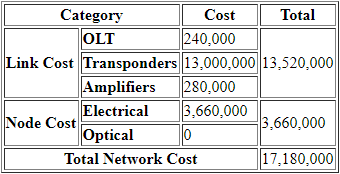
\includegraphics[width=10cm]{sdf/heuristic/figures/Low_Network_Cost_Opaque}
\caption{The low traffic network cost using Net2Plan.}
\label{Low_Network_Cost_Opaque}
\end{figure}

\begin{figure}[h!]
\centering
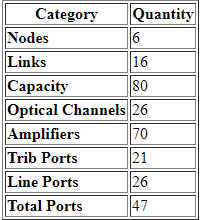
\includegraphics[width=5cm]{sdf/heuristic/figures/Low_Network_Info_Opaque}
\caption{The low traffic network info using Net2Plan.}
\label{Low_Network_Info_Opaque}
\end{figure}

\newpage
\textbf{Medium Traffic Scenario:}\\

Following all the steps mentioned in the previous subsection and using all the data referring to this scenario, the obtained result can be consulted in the following figure \ref{Medium_Network_Cost_Opaque}.

\begin{figure}[h!]
\centering
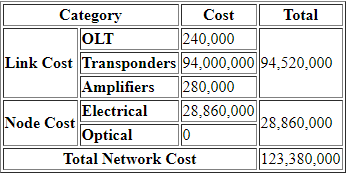
\includegraphics[width=10cm]{sdf/heuristic/figures/Medium_Network_Cost_Opaque}
\caption{The medium traffic network cost using Net2Plan.}
\label{Medium_Network_Cost_Opaque}
\end{figure}

\begin{figure}[h!]
\centering
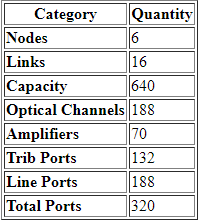
\includegraphics[width=5cm]{sdf/heuristic/figures/Medium_Network_Info_Opaque}
\caption{The medium traffic network info using Net2Plan.}
\label{Medium_Network_Info_Opaque}
\end{figure}

\newpage
\textbf{High Traffic Scenario:}\\

Following all the steps mentioned in the previous subsection and using all the data referring to this scenario, the obtained result can be consulted in the following figure \ref{High_Network_Cost_Opaque}.

\begin{figure}[h!]
\centering
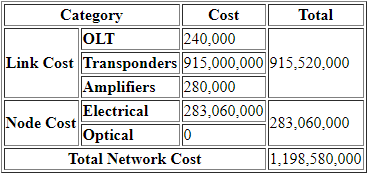
\includegraphics[width=10cm]{sdf/heuristic/figures/High_Network_Cost_Opaque}
\caption{The hight traffic network cost using Net2Plan.}
\label{High_Network_Cost_Opaque}
\end{figure}

\begin{figure}[h!]
\centering
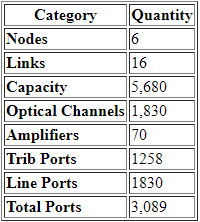
\includegraphics[width=5cm]{sdf/heuristic/figures/High_Network_Info_Opaque}
\caption{The high traffic network info using Net2Plan.}
\label{High_Network_Info_Opaque}
\end{figure}
